% Options for packages loaded elsewhere
\PassOptionsToPackage{unicode}{hyperref}
\PassOptionsToPackage{hyphens}{url}
%
\documentclass[
  9pt,
  ignorenonframetext,
]{beamer}
\usepackage{pgfpages}
\setbeamertemplate{caption}[numbered]
\setbeamertemplate{caption label separator}{: }
\setbeamercolor{caption name}{fg=normal text.fg}
\beamertemplatenavigationsymbolsempty
% Prevent slide breaks in the middle of a paragraph
\widowpenalties 1 10000
\raggedbottom
\setbeamertemplate{part page}{
  \centering
  \begin{beamercolorbox}[sep=16pt,center]{part title}
    \usebeamerfont{part title}\insertpart\par
  \end{beamercolorbox}
}
\setbeamertemplate{section page}{
  \centering
  \begin{beamercolorbox}[sep=12pt,center]{part title}
    \usebeamerfont{section title}\insertsection\par
  \end{beamercolorbox}
}
\setbeamertemplate{subsection page}{
  \centering
  \begin{beamercolorbox}[sep=8pt,center]{part title}
    \usebeamerfont{subsection title}\insertsubsection\par
  \end{beamercolorbox}
}
\AtBeginPart{
  \frame{\partpage}
}
\AtBeginSection{
  \ifbibliography
  \else
    \frame{\sectionpage}
  \fi
}
\AtBeginSubsection{
  \frame{\subsectionpage}
}
\usepackage{lmodern}
\usepackage{amsmath}
\usepackage{ifxetex,ifluatex}
\ifnum 0\ifxetex 1\fi\ifluatex 1\fi=0 % if pdftex
  \usepackage[T1]{fontenc}
  \usepackage[utf8]{inputenc}
  \usepackage{textcomp} % provide euro and other symbols
  \usepackage{amssymb}
\else % if luatex or xetex
  \usepackage{unicode-math}
  \defaultfontfeatures{Scale=MatchLowercase}
  \defaultfontfeatures[\rmfamily]{Ligatures=TeX,Scale=1}
\fi
\usetheme[]{Goettingen}
\usecolortheme{rose}
% Use upquote if available, for straight quotes in verbatim environments
\IfFileExists{upquote.sty}{\usepackage{upquote}}{}
\IfFileExists{microtype.sty}{% use microtype if available
  \usepackage[]{microtype}
  \UseMicrotypeSet[protrusion]{basicmath} % disable protrusion for tt fonts
}{}
\makeatletter
\@ifundefined{KOMAClassName}{% if non-KOMA class
  \IfFileExists{parskip.sty}{%
    \usepackage{parskip}
  }{% else
    \setlength{\parindent}{0pt}
    \setlength{\parskip}{6pt plus 2pt minus 1pt}}
}{% if KOMA class
  \KOMAoptions{parskip=half}}
\makeatother
\usepackage{xcolor}
\IfFileExists{xurl.sty}{\usepackage{xurl}}{} % add URL line breaks if available
\IfFileExists{bookmark.sty}{\usepackage{bookmark}}{\usepackage{hyperref}}
\hypersetup{
  pdftitle={BIOS6643 Longitudinal},
  pdfauthor={EJC},
  hidelinks,
  pdfcreator={LaTeX via pandoc}}
\urlstyle{same} % disable monospaced font for URLs
\newif\ifbibliography
\setlength{\emergencystretch}{3em} % prevent overfull lines
\providecommand{\tightlist}{%
  \setlength{\itemsep}{0pt}\setlength{\parskip}{0pt}}
\setcounter{secnumdepth}{-\maxdimen} % remove section numbering
\AtBeginSubsection{}
\AtBeginSection{}
\ifluatex
  \usepackage{selnolig}  % disable illegal ligatures
\fi

\title{BIOS6643 Longitudinal}
\subtitle{L18 Nonparametric}
\author{EJC}
\date{}
\institute{Department of Biostatistics \& Informatics}

\begin{document}
\frame{\titlepage}

\begin{frame}[allowframebreaks]
  \tableofcontents[hideallsubsections]
\end{frame}
\hypertarget{mixture-models}{%
\section{Mixture Models}\label{mixture-models}}

\begin{frame}{Topics involved with these notes:}
\protect\hypertarget{topics-involved-with-these-notes}{}
\begin{itemize}
\item
  Modeling mixture distributions
\item
  Zero-plus-continuous (or `clump at zero') data
\item
  2-part models
\item
  PROC NLMIXED
\end{itemize}

\vspace{\baselineskip}

\begin{itemize}
\item
  \textbf{Associated reading:}

  \begin{itemize}
  \tightlist
  \item
    related topics in course notes (see `Modeling independent or
    correlated non-normal data' chapter).
  \end{itemize}
\end{itemize}
\end{frame}

\hypertarget{zero-plus-continuous-mixture-distributions}{%
\section{Zero-plus-continuous mixture
distributions}\label{zero-plus-continuous-mixture-distributions}}

\begin{frame}{Zero-plus-continuous mixture distributions}
\protect\hypertarget{zero-plus-continuous-mixture-distributions-1}{}
Some distributions are more complex and cannot be modeled well using
standard methods. For example, some distributions have possibility of 0
but where positive values can be well-modeled as continuous. Some
examples:

\begin{itemize}
\item
  Health care costs.
\item
  Precipitation amounts.
\end{itemize}

Such a distribution is a discrete and continuous mixture, so both
aspects need to be accounted for properly.

Some possible distributions for the continuous part would be:
log-Normal, Gamma, Weibull, truncated normal.
\end{frame}

\begin{frame}{}
\protect\hypertarget{section}{}
With the cost example, some potential interesting questions are:

\begin{itemize}
\item
  What is the chance someone will incur a cost?
\item
  What is the mean of costs for those who do?
\item
  What is the overall mean, taking into account both sources (those who
  have some costs, and those who don't)?
\end{itemize}

\vspace{\baselineskip}

With the precipitation example, equivalent questions are:

\begin{itemize}
\item
  What is the probability of rain in a given city?
\item
  What is the mean rainfall on days when it did rain?
\item
  What is the overall mean rainfall in each city?
\end{itemize}
\end{frame}

\begin{frame}{}
\protect\hypertarget{section-1}{}
We can use the Theorem on Total Probability to derive the complete `0 +
continuous' distribution. Let \(R\) denote an indicator variable for
positive values of \(Y\) and let \(p\) denote the probability of a
positive value. Then we have

\(F_Y (y)=P(Y \leq y\ |\ r=0)P(R=0)+P(Y \leq y\ |\ r>0)P(R=1) =P(Y \leq y\ |\ r=0) (1-p)+P(Y \leq y\ |\ r=1) p =(1-p) I_{y=0}+p F_{Y\ |\ r=1} (y\ |\ r=1)\);
where \(F_{Y\ |\ r=1} (y\ |\ r=1)\) is the CDF of a random variable with
positive density for positive values of \(Y\) (e.g., Weibull, Gamma,
log-Normal).

Although the CDF is easier to work with for mixed distributions, we need
the PDF for the likelihood. The form can be defined mathematically as
\(f_Y (y)=(1-p) \delta_0 (y)+p f_{Y\ |\ r=1} (y\ |\ r=1)\)

where \(\delta_0 (y)\) is the Dirac delta function, defined to be 0 when
\(y \neq 0\) but integrates to 1 over all y on the real line. For
practical purposes (e.g., in the likelihood function) we set this term
to 1 so that \(f_Y (y)=(1-p) I_{r=0}+p f_{Y\ |\ r=1} (y\ |\ r=1)\)
\end{frame}

\begin{frame}{}
\protect\hypertarget{section-2}{}
In our example with rainfall, we'll consider the Gamma distribution for
positive amounts (i.e., given \(R=1\)), which has density

\(f_Y (y)= \frac {x^{\theta -1} e^{-x/ \lambda)}} {\lambda^\theta \Gamma (\theta )},\ for\ y>0\);
where \(\theta >0\) is a shape parameter and \(\lambda>0\) is a scale
parameter.

The mean of this distribution is \(\theta \lambda\) and the variance is
\(\theta \lambda^2\).
\end{frame}

\begin{frame}{}
\protect\hypertarget{section-3}{}
We can define a mixed model for this mixed distribution as follows.

\begin{itemize}
\item
  Occurrence model: \(logit(p_{ij})=\alpha_0+b_{0i}\), where
  \(p_{ij}=P(Y_{ij}=1\ |\ b_{0i})\).
\item
  Intensity model:
  \(Y_{ij} \ |\ r=1,\ b_{1i},\ b_{2i} \sim \mathcal {Gamma} (\theta +b_{1i},\ \lambda+b_{2i} )\)
\item
  Covariance structure of random effects:
  \(\pmb b=(b_{0i},\ b_{1i},\ b_{2i} )^{\top} \sim \mathcal N(\pmb 0,\ \pmb G)\),
  where \(\pmb G\) is a \(3 \times 3\) unstructured matrix.
\end{itemize}

The addition of random intercepts to both shape and scale parameters for
each city allows unique Gamma rainfall distribution by city.
\end{frame}

\begin{frame}{Deriving the mean, variance and covariance}
\protect\hypertarget{deriving-the-mean-variance-and-covariance}{}
For our model,
\(E[Y_{ij} \ |\ \pmb b]=E\big[E[Y_{ij} \ |\ \pmb b,\ r]\big] = 0(1-p_{ij})+ \mu_{ij+} p_{ij}=p_{ij} \mu_{ij+}\)
where \(\mu_{ij+}\) is the mean of the positive \(Y\) values and
\(p_{ij}\) is the probability of a positive value. Now
\(p_{ij}=\frac 1 {1+exp (-\alpha _0-b_{0i}^p)}\)) and
\(\mu_{ij+}=(\theta +b_{0i}^{shape})(\lambda+b_{0i}^{scale})\); (where
conditioning on random effects is implied). Thus the mean that puts the
0's and positive data together is
\(E[Y_{ij} \ |\ \pmb b]= \frac {(\theta +b_{0i}^{shape})(\lambda+b_{0i}^{scale})} {1+exp (-\alpha _0-b_{0i}^p)}\).

It may be just as meaningful to jointly report \(p_{ij}\) and
\(\mu _{ij+}\), which represent the probability of rain or snow on day
\(j\) for city \(i\) and the average precipitation over days when it did
rain/snow.
\end{frame}

\begin{frame}{}
\protect\hypertarget{section-4}{}
We can also derive
\(Var[Y_{ij} \ |\ \pmb b]=p_{ij} ( \sigma _{ij+}^2+ \mu_{ij+}^2 (1-p_{ij}))\),
where \(\sigma _{ij+}^2\) is the variance of the positive \(Y\) values
(show for homework).

Covariance and correlation:

\(Cov(Y_{ij},\ Y_{ik})=E\big[Cov[Y_{ij},\ Y_ik \ |\ \pmb b]\big]+Cov\big[E[Y_{ij} \ |\ b],\ E[Y_{ik} \ |\ \pmb b]\big]\)

\begin{itemize}
\item
  The second term is straightforward to determine since we have already
  defined the model in terms of mean responses given the random effects.
\item
  The first term is more difficult since
  \(Cov[Y_{ij},\ Y_{ik} \ |\ \pmb b]\) does not come directly from the
  defined model. Specifically, no error term is defined for the model.
  (For an LMM, it would be the \((i,\ j)\)th element of the error
  covariance matrix, \(\pmb R_i\).) We could employ residuals to
  estimate the quantity. Check.
\end{itemize}
\end{frame}

\begin{frame}{}
\protect\hypertarget{section-5}{}
For the (straightforward) term on the right side,

\(Cov\big[ E[Y_{ij} \ |\ \pmb b),\ E[Y_{ik} \ |\ \pmb b]\big]=Cov[\mu_{ij+} p_{ij},\ \mu _{ik+} p_{ik}]=Cov\Big[\frac {(\theta +b_{1i})(\lambda+b_{2i})} {1+exp (-\alpha _0-b_{0i})},\ \frac {(\theta +b_{1i})(\lambda+b_{2i})} {1+exp(-\alpha_0-b_{0i})} \Big]\)

where
\(\pmb b=(b_{0i},\ b_{1i},\ b_{2i} )^{\top} \sim \mathcal N(\pmb 0,\ \pmb G)\),

\[
\pmb G=
\begin{pmatrix}
\sigma _{b_0^p}^2&& \\ 
\phi_{21}  \sigma_{b_0^p}   \sigma _{b_0^{shape}}& \sigma _{b_0^{shape}}^2& \\ \phi_{31}  \sigma _{b_0^p}   \sigma _{b_0^{scale}}&\phi_{32}  \sigma _{b_0^{shape}}   \sigma _{b_0^{scale}} & \sigma _{b_0^{scale}}^2 
\end{pmatrix}
\]

Here we use an unstructured G matrix and formulate the model so that the
correlation parameters are directly estimated. Note that covariances
depend on city \(i\) but not day \(j\) since we only have random
intercepts in the model (but we keep both subscripts on parameters for
potential generalizations). To make a time-dependent structure, we could
add fixed and random effects for day in the model (in the intensity
and/or occurrence parts). For models I tried it did not seem to help.
\end{frame}

\begin{frame}{}
\protect\hypertarget{section-6}{}
Here is the analysis of rainfall data in 6 cities selected from across
the U.S. Note that this is more of a demonstration of methods; cities
were not randomly selected and more advanced time-series models might be
used for actual analysis. But it is real data and the modeled
distribution appears to fit the data well.

The cities: Atlanta, Aurora, Chicago, Houston, New York, Phoenix,
Sacramento, Seattle. These are the `subjects'.

Data collection time frame: first 100 days of 2017.

Outcome variable: precipitation, measured in inches.
\end{frame}

\begin{frame}{}
\protect\hypertarget{section-7}{}
SAS code and output follow. Note that the names given in the SAS code
are consistent with the quantities shown above, just written out instead
of in Greek symbols.

\begin{center}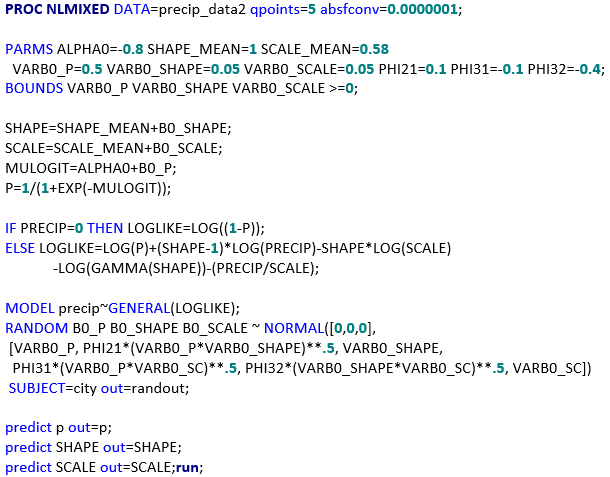
\includegraphics[width=1\linewidth]{figs_L18/f1} \end{center}
\end{frame}

\begin{frame}{}
\protect\hypertarget{section-8}{}
\begin{center}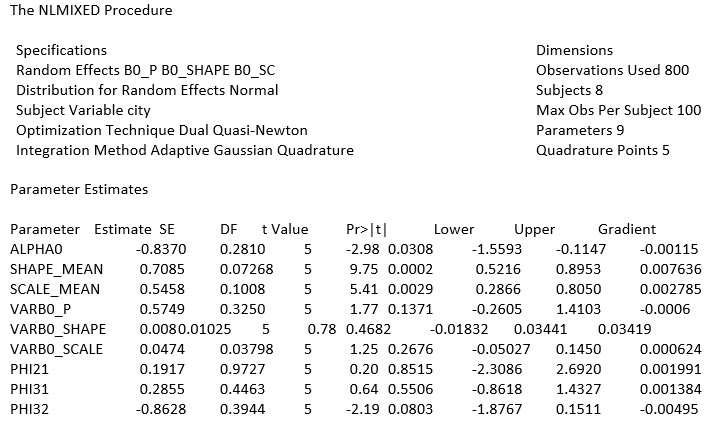
\includegraphics[width=1\linewidth]{figs_L18/f2} \end{center}
\end{frame}

\begin{frame}{}
\protect\hypertarget{section-9}{}
We could also add a fixed or fixed and random effect for day in either
the Occurrence or Intensity models (or both), which would induce a
slightly more time-sensitive correlation structure. However for the data
at hand, such additions did not improve the model fit.

Predicted values that include random effect variations are obtained by
the `predict' statements given at the end of the SAS code. Here is some
additional code that gets quantities of interest (\(p_{ij}\),
\(\mu_{ij+}\), and \(\mu_{ij}\))
\end{frame}

\begin{frame}{}
\protect\hypertarget{section-10}{}
The graph below shows overall means for each city using both descriptive
statistics and the model-based approach. They are generally in
agreement.

\begin{center}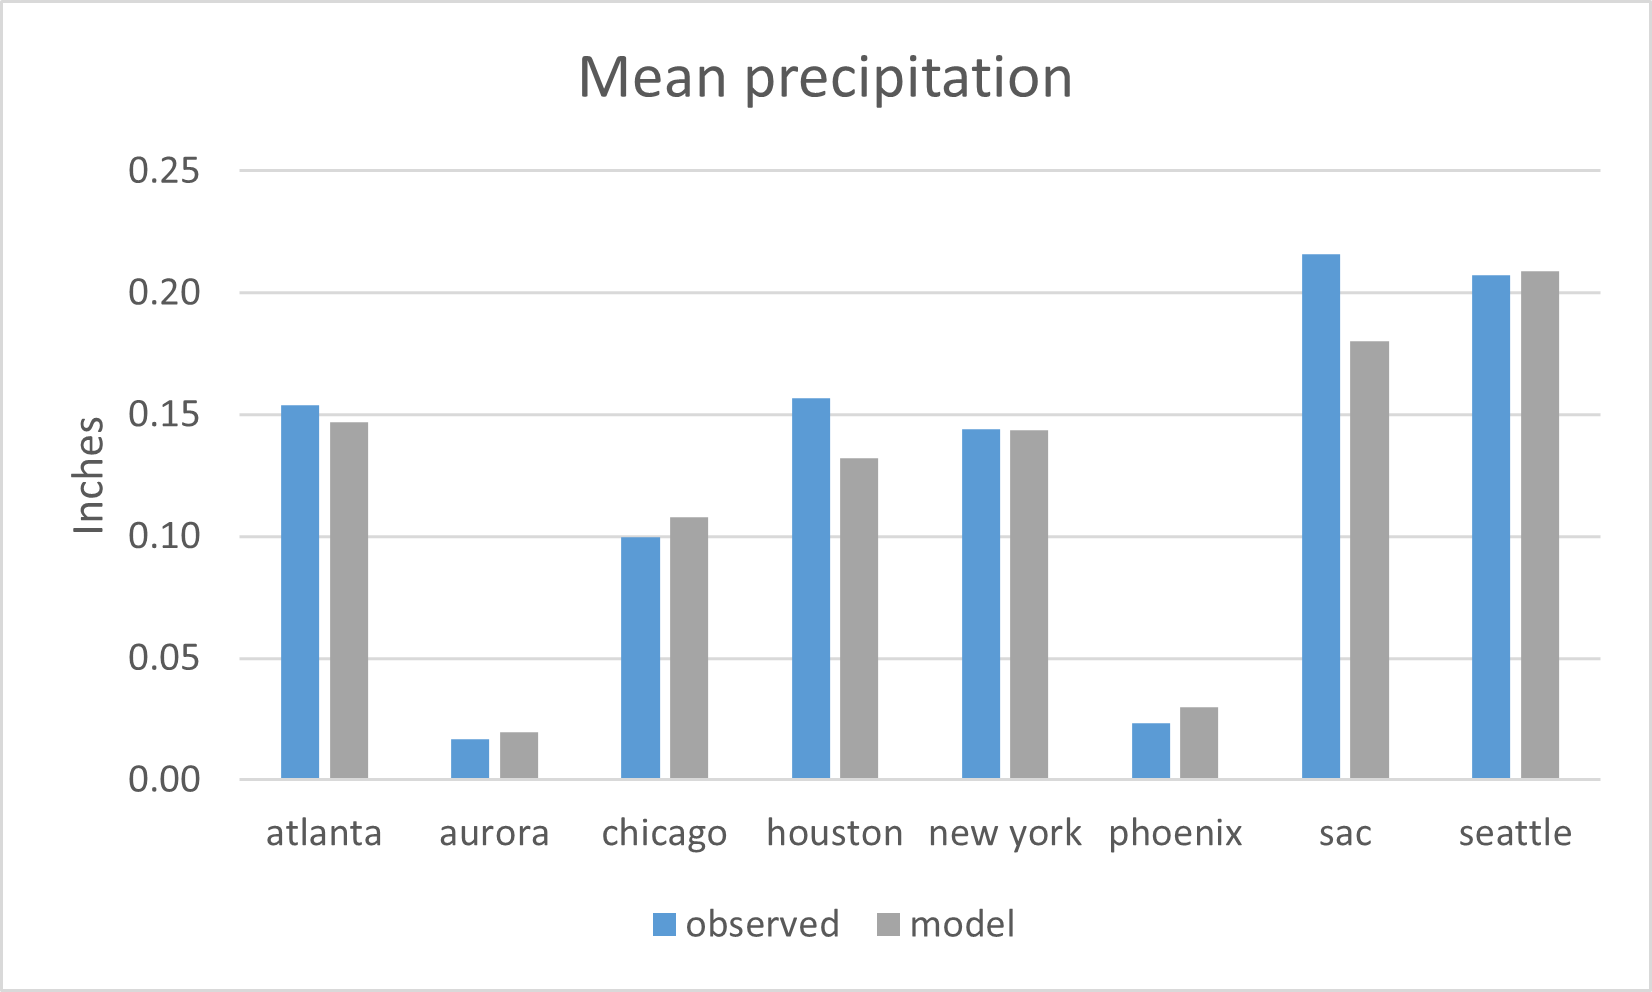
\includegraphics[width=0.5\linewidth]{figs_L18/f4} \end{center}
\end{frame}

\begin{frame}{}
\protect\hypertarget{section-11}{}
The graphs below show how modeled values of
\(\mu_{ij} \ |\ b_{1i},b_{2i}\) and \(p_{ij} \ |\ b_{0i}\) versus
descriptive quantities. These graphs demonstrate how information is lost
when we only consider mean precipitation as in the last graph. For
example, Seattle has greater likelihood of rain on any given day, but
when we restrict to days where it did rain, Sacramento and Houston had
higher mean daily precipitation amounts. Note that modeled amounts by
city tend to exhibit shrinkage towards to overall mean (a bit higher for
drier cities; less for wetter cities) which is expected for empirical
Bayes estimates.

\begin{center}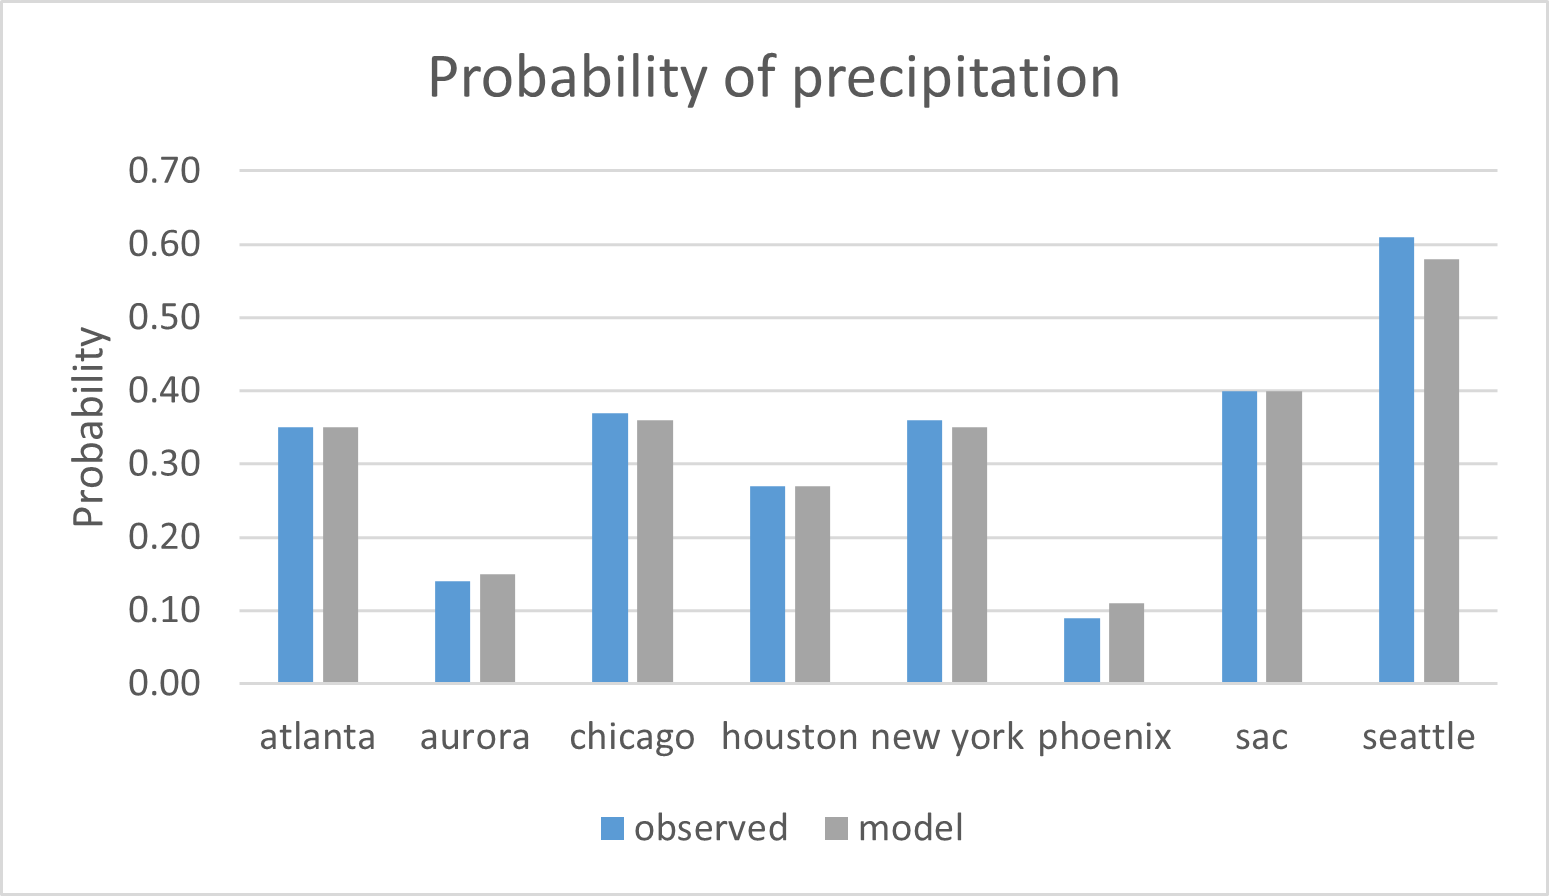
\includegraphics[width=0.5\linewidth]{figs_L18/f5} \end{center}

\begin{center}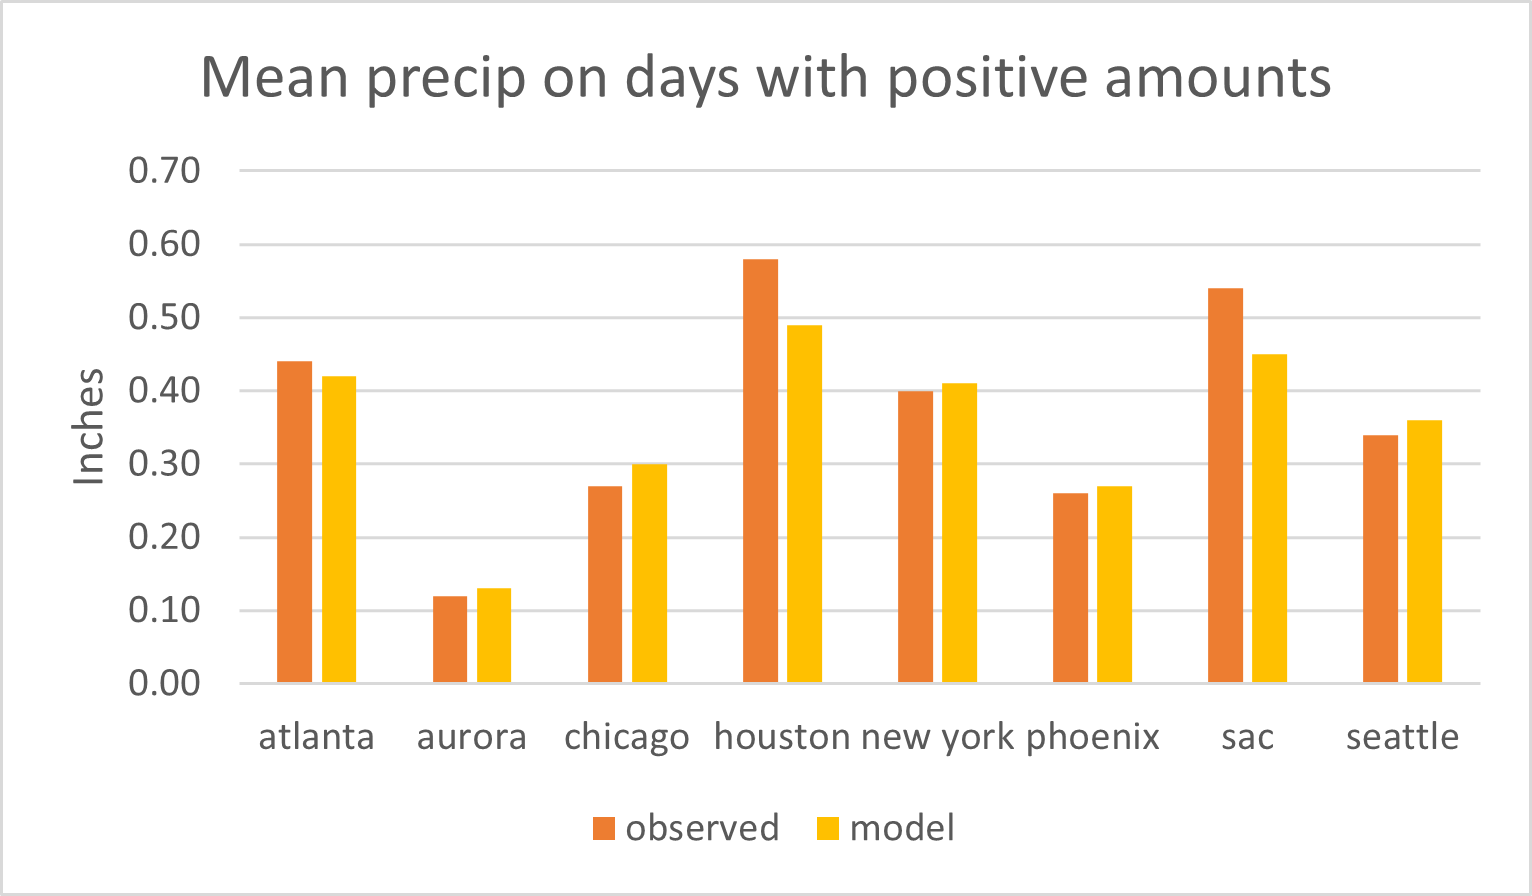
\includegraphics[width=0.5\linewidth]{figs_L18/f6} \end{center}
\end{frame}

\begin{frame}{}
\protect\hypertarget{section-12}{}
Important note: historical data might yield somewhat different results.
Here we only used the early part of 2017 to build the model, so
inference should be restricted to `around this time or times that are
similar in climate' and during winter.

One might wonder why the model approach is of any use, since we can
estimate these quantities directly. Remember that we additionally can
address correlation in our model. Also, the modeling approaches allows
for the addition of other covariates and random effects, if we so wish.

Given that probabilities and means were not time sensitive in our given
model, the correlation between responses should be somewhat like the
compound symmetric structure.
\end{frame}

\begin{frame}{Other mixture distributions}
\protect\hypertarget{other-mixture-distributions}{}
The previous example involved a mixture of a discrete and continuous
distributions. The same principle can be used when mixing discrete
distributions or mixing continuous distributions. In fact, mixing
like-type distributions is probably easier, particularly when mixing
discrete distributions.

A zero-inflated Poisson (ZIP) takes a standard Poisson distribution,
and, as the name implies, adds to the probability of 0 occurring. This
is obtained by mixing a degenerate distribution with point mass of one
at zero, with a standard Poisson.

The random variable \(Y\) with ZIP distribution (Lambert, 1992) can be
summarized as follows.

\(Y \sim 0\) with probability \(p\)
\(Y \sim \mathcal {Poisson}(\lambda)\) with probability \(1-p\)
\end{frame}

\begin{frame}{}
\protect\hypertarget{section-13}{}
The distribution has a binomial process (whether or not \(Y\) is 0) and
a count process, associated with the Poisson distribution. However,
there are two ways in which a `0' can be obtained; one is by sampling
from the Poisson, and one is by the added 0 element. For some
applications, it may be meaningful to distinguish these two types of
zeroes, which is discussed in the last slides of this set.

Given the ZIP formulation above, we can combine the information to write
a specific probability mass function:

\(Y=0\) with probability \(p+(1-p)e^{-\lambda}\) \(Y=k\) with
probability \((1-p) e^{-\lambda}\lambda^k/k!,\ for\ k=1,\ 2,\ ...\)
\end{frame}

\begin{frame}{}
\protect\hypertarget{section-14}{}
If desired, models can specify correlation between parameters \(p\) and
\(\lambda\). Similar approaches can also be used to construct
zero-inflated negative binomial (ZINB) and zero-inflated binomial (ZIB)
models.

Mixing continuous distributions can also be performed. For example,
mixing of normal distributions has been suggested to obtain more complex
distributions for random effects in mixed models (see `Heterogeneity
Models' in Verbeke and Molenberghs, Linear Mixed Models for Longitudinal
Data, 2000).
\end{frame}

\begin{frame}{Additional thoughts.}
\protect\hypertarget{additional-thoughts.}{}
Mixture distributions may be useful even if the distribution is
completely discrete or continuous. For example, a zero-inflated Poisson
distribution takes a standard Poisson and then adds a binomial random
variable such that the probability that the mixed random variable takes
on a value of 0 is increased.

We can also define mixture models based on how values in the mixture can
be distinguished with respect to structure and sampling.
\end{frame}

\begin{frame}{Hurdle models versus zero-inflated models}
\protect\hypertarget{hurdle-models-versus-zero-inflated-models}{}
From McDowell (2003): A hurdle model is ``a modified count model in
which the two processes generating the zeros and the positives are not
constrained to be the same'' (Cameron and Trivedi 1998). Mullahy (1986)
states, ``The idea underlying the hurdle formulations is that a binomial
probability model governs the binary outcome of whether a count variate
has a zero or a positive realization. If the realization is positive,
the ``hurdle is crossed'', and the conditional distribution of the
positives is governed by a truncated-at-zero count data model.

A zero-inflated model is one where the 0's could come from 2 different
types of processes (structural and sampling), and the 0's versus
nonzero's are not governed by one overlying Bernoulli process. So, for
example, we have a Poisson process, which could include 0's and positive
integers, but then is also a structural source for the 0's.
\end{frame}

\begin{frame}{}
\protect\hypertarget{section-15}{}
As an example, consider a type of number of packs of cigarettes smoked
in the last week. For smokers, most will likely smoke, but there is the
chance that some will not; these will be `sampling 0's'; but if the
cohort also includes non-smokers, then those would be structural 0's
since, by definition, they do not smoke. This would be an example of a
zero-inflated model.

However, say that the time frame considered is much longer, like 3
months. In this case, it may be reasonable to assume that 0's only come
from non-smokers and positive values come from smokers. We might use a
hurdle model in this case.
\end{frame}

\begin{frame}[fragile]{}
\protect\hypertarget{section-16}{}
Consider a model that needs to account for added 0's (either zero
inflated, or via hurdle model). For simplicity of notation, let
\(p=P(Y=0\ |\ z,\ \gamma)\). Also f may represent either a pdf or pmf,
depending on whether the distribution of positive values is continuous
or discrete.

\begin{verbatim}
For a zero-inflated model, we have $f_ZIP (x,\ z,\ \beta,\ \gamma)=p_{z,\ \gamma } I_{0}(y) + (1-p_{z,\ \gamma}) f_{count} (y\ |\ x,\ \beta)I_{0,\ 1,\ 2,\ ...} (y)$

For a hurdle model, we have 
\end{verbatim}

\[
f_{hurdle} (x,\ z,\ \beta,\ \gamma)=
\begin{cases}
p_{z,\ \gamma} &  y=0 \\ 
(1-p_{z,\ \gamma}) \frac {f_{count} (y\ |\ x,\ \beta)} {(1-f_{count} (0\ |\ x,\ \beta))} & y>0
\end{cases}
\]
\end{frame}

\begin{frame}{}
\protect\hypertarget{section-17}{}
The primary difference between models is that for the ZIP model, we have
a standard distribution (\(f_count\)), such as a Poisson distribution
and add some 0's to it, while for the hurdle model, we distinguish
modeling of the 0's versus modeling of the positive values based on
their structural differences. In order to model the positive values, we
take a standard distribution like the Poisson and truncate it so that a
value of 0 has no positive probability/mass.

Going back to the rainfall application, we combined a discrete and
continuous model, the latter of which already does not have any
probability mass on 0 (no need to truncate it). In this sense we
intrinsically have a hurdle model. It may also make sense theoretically
if there are not `structural' and `sampling' 0's.
\end{frame}

\begin{frame}{}
\protect\hypertarget{section-18}{}
However a zero-inflated model might make sense theoretically if there is
some condition considered. For example, clouds must be present for rain
or snow. But precipitation is not guaranteed when clouds are present.
Thus, 0's could be distinguished by those on sunny (structural) and
cloudy (sampling) days. One model governs rainfall when it is cloudy,
and one whether it is cloudy or sunny. For the `cloudy' model, we'd need
some distribution that allows positive probability for 0 but also for
positive values. A count-type model might work if we categorize the
precipitation levels.

In some cases we may not need to consider the theoretical constructs of
zero and nonzero values. We may use a model and be more concerned with
how accurate the distribution is, and not estimate parameters based on
distinguishing sampling versus structural-based zeroes.
\end{frame}

\end{document}
